\documentclass{SBCbookchapter}
\usepackage[utf8]{inputenc}
\usepackage[T1]{fontenc}
\usepackage[brazil,english]{babel}
\usepackage{graphicx}
\title{Face Recognition}
\author{}
\begin{document}
\maketitle

%\addcontentsline{toc}{chapter}{Statistics}

%\emph{Find a statistical method which uses only Japan Meteorological Agency (JMA) best track typhoon data during or before year $n$ to hind-cast the entire best track of all typhoons in years $n+1$.   Given only the latter typhoons' initial three best track points (i.e. at $t=0,6,$ and $12$ hours), the maximum position error at each hind-casted track point must be less than 500 km. The method must work for the three most recent years of published best track data.}

\vspace{.3in}
\begin{minipage}[r]{4.25in}{\small
  Child trafficking is a heinous crime which should be combatted by all means including advanced technology.  In the case of trans-national
  trafficking, border control may utilize face recognition technology to aid in the rescue of trafficked children.}
  \end{minipage}

\newpage

\section{Introduction}

\section{Face Recognition}
Face recognition is a type of object recognition, which is a subfield of image recognition (Figure \ref{fig1}). Face recognition itself may be classified by the methods employed (Table \ref{tab1}).

\begin{figure}[h]
\centering
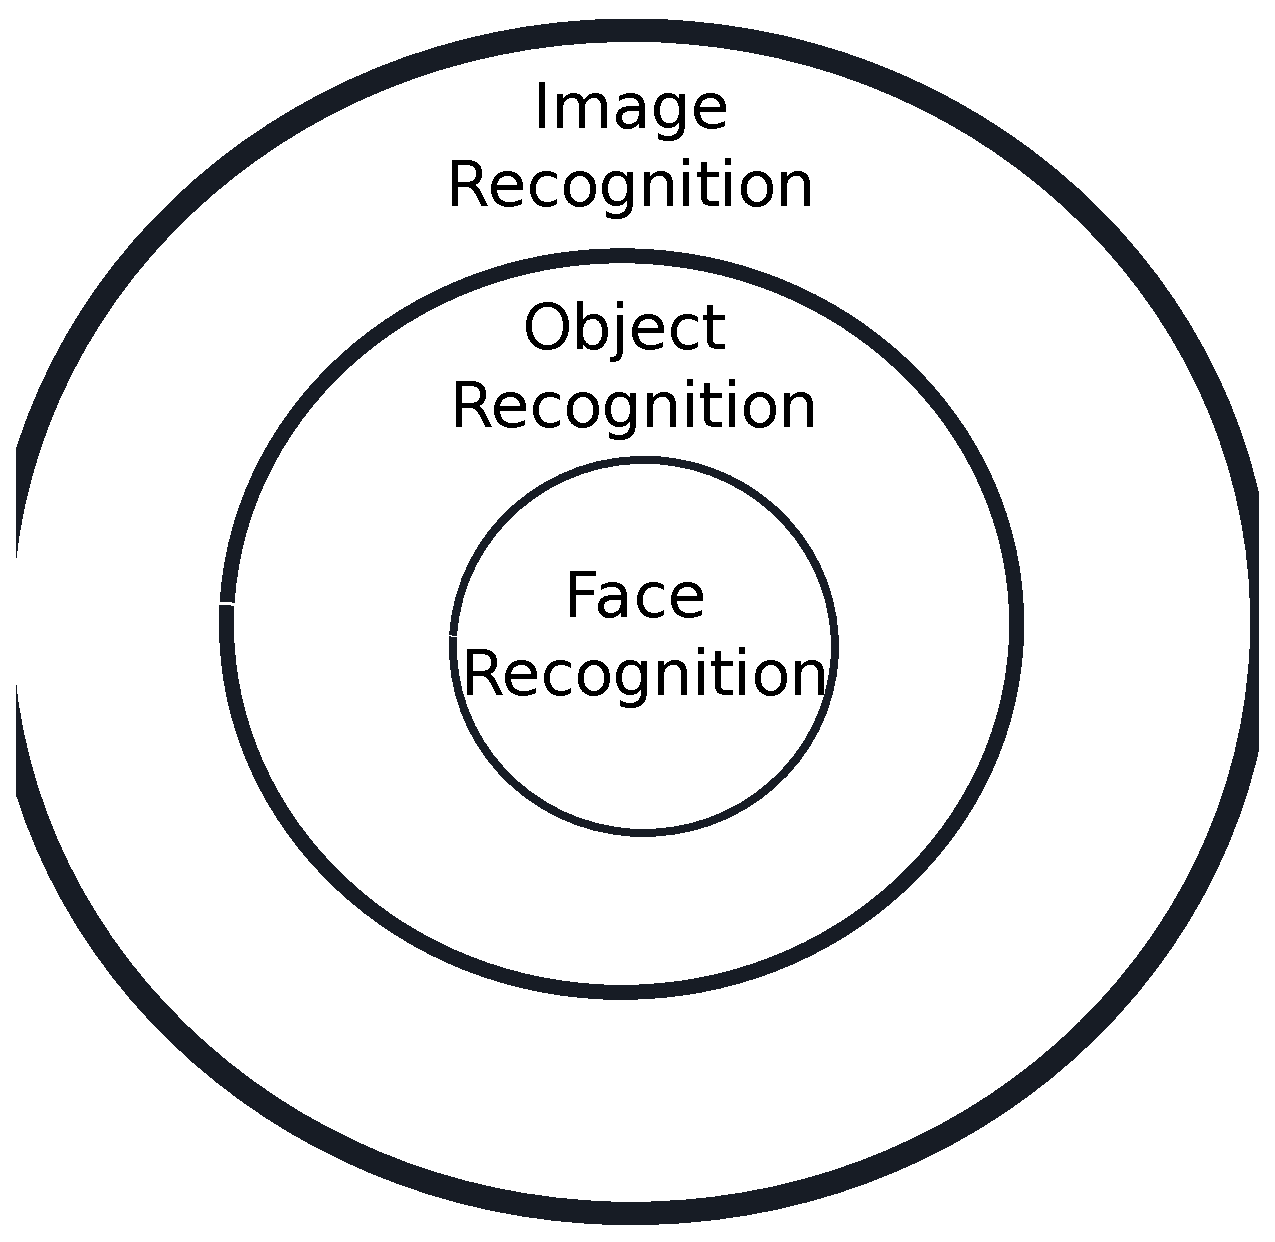
\includegraphics[width=1in, height=1in]{fig1.eps}
 \caption{Face recognition as a subfield of object and image recognition.}
 \label{fig1}
\end{figure}


    \begin{table}[h]
\centering
\tiny
\begin{tabular}{|c|c||}\hline
CRITERIA & TYPES \\\hline
Algorithm & linear, non-linear\\
Consideration of Face Category Information& supervised, semi-supervised, unsupervised\\
Data architecture& local, global\\\hline
 \end{tabular}
  \caption{Classification of Face Recognition \cite{Gong}}
  \label{tab1}
\end{table}



\section{Computer Project}
Write a program which can





\vspace{1in}

\emph{Acknowledgement:}
.
\vspace{.25in}

\emph{Project Team:}

\newpage
 \begin{thebibliography}{9}

 \bibitem{Gong}  {\sc  GONG, S., LIU,C., ZHONG, B., LI, Y., DONG, H.}, 2019. {\em Advanced Image and Video Processing Using MATLAB (Modeling and Optimization in Sience and Thecnologies Book 12)},. Springer-Verlag,  pp.

\bibitem{Chan} {\sc CHAN, J.C.L.}, 2005: The physics of tropical cyclone motion. \emph{Annu. Rev. Fluid Mech.} {\bf 37}, 99-128.

\end{thebibliography}


\end{document}